\begin{surferPage}[萊布斯7次曲面]{萊布斯7次曲面}
2004年,奧利弗萊布斯在美因茨大學完成他的學位論文時構造了一個$7$次曲面。這是$7$次曲面的當今世界紀錄。但是,仍然
有可能存在$104$個奇異點的$7$次曲面。 萊布斯的曲面具有正$7$邊形(左圖)的對稱性。這可以從曲面的頂部觀察到(右圖)

    \vspace*{-0.3em}
    \begin{center}
      \begin{tabular}{c@{\qquad}c}
        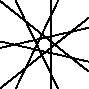
\includegraphics[height=1.5cm]{./../../common/images/labsseptic1.pdf}
        &
        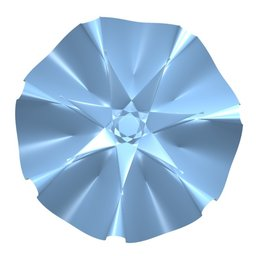
\includegraphics[height=1.5cm]{./../../common/images/labs_septic_von_oben}
      \end{tabular}
    \end{center}
    \vspace*{-0.3em}

為了構造這個曲面,奧利弗萊布斯利用了計算代數幾何以及奇異點中流行的計算機系統{\sc Singular}(凱撒斯勞滕大學)。
我們知道時鐘的規則是:24.00$=$0.00, 24.00 $+$ 1 小時是1點,而不是25點。這種有限集上的自然計算規則同樣被奧利弗萊布斯加以利用。
\end{surferPage}
